\section{計算}\label{s1:計算} %{
\subsection{ベータ関数}\label{s2:ベータ関数} %{
$0<\Re x,\; 0<\Re y$に対してベータ関数$B(x,y)$は次のように定義される。
\begin{equation}\label{eq:Beta}
	B(x, y) := \int_0^1 \frac{dt}{t(1-t)}t^x(1-t)^y
	\quad\text{for all } 0<\Re x,\; 0<\Re y
\end{equation}

ベータ関数とガンマ関数は次の関係にある。
\begin{equation}
	B(x, y) = \frac{\Gamma(x)\Gamma(y)}{\Gamma(x+y)}
	\quad\text{for all } 0<\Re x,\; 0<\Re y
\end{equation}
\begin{proof} %{
	定義\eqref{eq:Beta}の積分変数を$s:=t/(1-t)$と変換すると、ガンマ関数の
	積分表示が現れる。
	\begin{alignat*}{2}
		B(x, y) &= \int_0^\infty\frac{ds}{s}\frac{s^x}{(1+s)^{x+y}}
		&\quad&\text{// } s := \frac{t}{1-t} \\
		&= \frac{1}{\Gamma(x+y)}\int_0^\infty\frac{ds}{s}s^x
		\int_0^\infty\frac{du}{u}u^{x+y}e^{-(1+s)u}
		&\quad&\text{// } \Gamma(x) = a^x\int_0^\infty\frac{dt}{t}t^xe^{-at} \\
		&= \frac{1}{\Gamma(x+y)}\int_0^\infty\frac{du}{u}u^{x+y}e^{-u}
		\int_0^\infty\frac{ds}{s}s^xe^{-su} \\
		&= \frac{\Gamma(x)}{\Gamma(x+y)}\int_0^\infty\frac{du}{u}u^ye^{-u} \\
		&= \frac{\Gamma(x)\Gamma(y)}{\Gamma(x+y)}
	\end{alignat*}
\end{proof} %}

定義\eqref{eq:Beta}の積分路を変形して、$y$の実部が負の場合に解析接続しよう。
$C$を図\ref{fig:ベータ関数の積分路その一}の積分路とすると、次の式が成り立つ。
\begin{equation*}
	B(x,y) = \frac{1}{1 - e^{-2\pi iy}}\int_C \frac{dt}{t(1 - t)}t^x(1 - t)^y
	\quad\text{for all } 0 < \Re x,\; 0 < \Re y,\; y\not\in\sei
\end{equation*}
ここで、複素平面の分岐切断は、$x\in\sei$の時は$(-\infty,1)$、$x\not\in\sei$
の時は$(0,1)$とする。

\begin{figure}[htbp] %{
	\begin{center}
		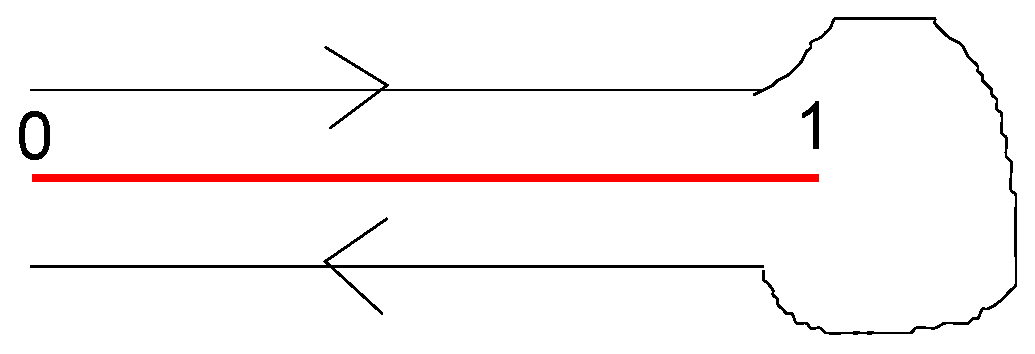
\includegraphics[width=0.3\textwidth]{fig/contour-2.eps}
	\end{center}
	\caption{ベータ関数の積分路その一}\label{fig:ベータ関数の積分路その一}
\end{figure} %}
%s2:ベータ関数}
\subsection{ベータ関数の和}\label{s2:ベータ関数の和} %{
$0<\Re a$かつ$0<\Re b$とすると、次の式が成り立ち、
\begin{equation*}
	\sum_{n\in\sizen}B(n + a, b)x^n 
	= \int_0^1 \frac{dt}{t(1 - t)}t^a(1 - t)^b \sum_{n\in\sizen}(tx)^n
	= \int_0^1 \frac{dt}{t(1 - t)}\frac{t^a(1 - t)^b}{1 - xt}
\end{equation*}
次の式が得られる。
\begin{equation*}\begin{split}
	\sum_{n\in\sizen}B(n + a, b) = B(a, b - 1) 
\end{split}\end{equation*}
%s2:ベータ関数の和}
\subsection{二項係数の計算}\label{s2:二項係数の計算} %{
任意の$0<k\in\jitu,\;x\in\Ballx{0}{1}$に対して次の式が成り立つ。
\begin{equation}\label{eq:分数の二項係数}
	(1 - x)^{-k} = \sum_{n\in\sizen}\frac{x^n\Gamma(k+n)}{n!\Gamma(k)}
	= \sum_{n\in\sizen}\frac{x^n}{(n + k)B(n + 1, k)}
\end{equation}
$k\in\fukuso$でも成り立つと思うが、その場合は解析接続が必要になる。
%s2:二項係数の計算}
%s1:計算}
